\section{Aplicando MDD al Desarrollo de un Sistema de Venta de Libros por Internet}

Mostraremos como el modelo PIM de ese sistema es automaticamente transformado en un PSM considerablemente complejo y luego veremos como finalmente se llega al codigo ejecutable. La complejidad del ejemplo es considerable, sin embargo nos enfocaremos solo en una parte reducida pero suficientemente completa como para apreciar los detalles del proceso. En las siguientes secciones introduciremos los requisitos del sistema que tomamos como ejemplo y describiremos los modelos y transformaciones involucrados en su desarrollo

\subsection{El Sistema de Venta de Libros por Internet}


Libros por Internet, al estilo Amazon, que permite vender y comprar libros a través de Internet. Hemos instalado el ejemplo completo en el sitio http://www.lifia.info.unlp.edu.ar/bookstore. Los requisitos generales del sistema son los siguientes: 
1. El bookstore será un sistema basado en la web para la venta de libros.
2. El bookstore tiene libros de los que se conoce el nombre, descripción, los autores, el precio. 
Los libros están organizados por categorías. Un ejemplo para categorías puede ser novelas, cuentos, historia. Un mismo libro puede tener varias versiones, algunas impresas y otras digitales. De los impresos se conoce el tamaño físico, la presentación, el stock y el peso para el envío. De los digitales su tamaño en bytes y el formato del archivo que lo contiene. La presentación impresa puede ser de tapa dura, edición de lujo, etc.
3. El usuario debe poder agregar libros en un carrito de compras online, previo a realizar la compra. Al momento de finalizar la compra, se generará una orden que incluye los ítems agregados al carrito de compras. Una vez confirmada la orden, se le enviará un mail al usuario informándole los datos de la misma. Similarmente, el usuario debe poder sacar ítems de su carrito o actualizar las cantidades de un ítem pedido. 
4. El usuario debe ser capaz de mantener una lista con los libros que desea comprar más tarde. 
5. El usuario debe poder cancelar órdenes antes de que hayan sido enviadas. 
6. El usuario debe poder pagar con tarjeta de crédito o transferencia bancaria. 
7. El usuario podría devolver libros que ha comprado. 
8. El usuario debe poder crear una cuenta, de forma tal que el sistema recuerde sus datos (nombre de usuario, nombre y apellido, dirección, email, detalles de su tarjeta de crédito) en el momento de registrarse
9. El usuario debe ser capaz de buscar libros usando distintos métodos de búsqueda –título, autor, palabra clave o categoría– y luego podrá ver los detalles  de los resultados de su búsqueda. 
10. El usuario debe poder escribir una opinión acerca de sus libros favoritos. Las opiniones aparecerán junto con los detalles del libro.


\subsection{5.2 Aplicando MDD}

Identificaremos las partes del proceso de desarrollo de software que tienen especial significado dentro del framework MDD. Para comenzar debemos identificar el modelo PIM de nuestro sistema y luego debemos identificar cuáles son los modelos PSM y el código que se espera como resultado del proceso de desarrollo. También es necesario que definamos cuáles son las transformaciones que usaremos para generar el PSM y el código a partir del modelo PIM
Entonces, necesitamos construir un sistema basado en la web que satisfaga los requisitos planteados.

\begin{figure}[H]
\centering
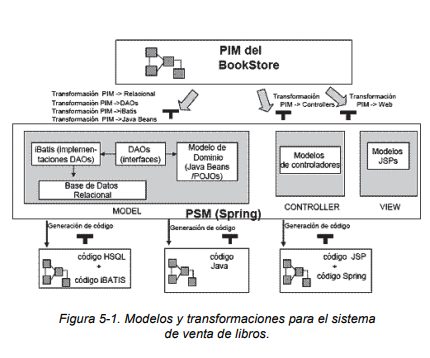
\includegraphics[scale=0.9]{./Imagenes/modelo20}
\caption{Ejemplo de figura 20}
\label{figura20}
\end{figure}


\subsection{5.2.1 El PIM y el PSM}

El primer paso en el proceso MDD consiste en la construcción de un modelo independiente de la plataforma (PIM) que describa (represente o modele) al sistema de venta de libros. Hemos elegido el lenguaje UML extendido mediante perfiles para expresar nuestro PIM. Se aplicaron los siguientes perfiles: MVC, Model, View y Session. En la figura 5-2 puede verse la definición de cada uno de ellos

\begin{figure}[H]
\centering
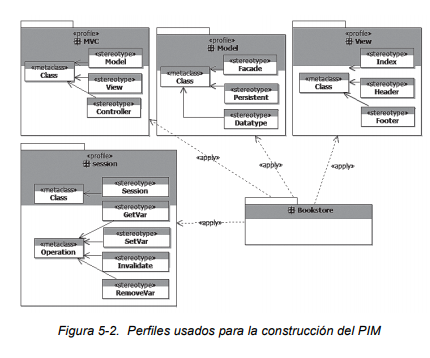
\includegraphics[scale=0.9]{./Imagenes/modelo21}
\caption{Ejemplo de figura 21}
\label{figura21}
\end{figure}

\subsection{5.2.2 La transformación de PIM a PSM }

El PSM tiene una arquitectura Model-View-Controller de tres capas, por lo tanto definiremos transformaciones separadas desde el PIM a cada parte del PSM.
Una transformación de PIM a la capa Model del MVC. La capa model a su vez está estructurada en distintos niveles, ya que distingue a los objetos del dominio en sí mismos (POJOs), a los mecanismos de acceso a los datos y a los mecanismos de persistencia de los datos (base de datos)

\subsection{5.2.3 La transformación de PSM a Código}

El siguiente paso consistirá en generar código ejecutable para cada PSM. Dado que en el framework MDD el código también es considerado un modelo, podemos hablar de modelos de código escritos en algún lenguaje de programación. Para el sistema de venta de libros por Internet tenemos varios modelos de código, escritos en HSQL, XML, Java y JSP. Por lo tanto necesitamos escribir al menos tres transformaciones de PSM a código: Una transformación de modelos relacionales a HSQL: una transformación que toma como entrada un modelo relacional y produce el script necesario para crear las tablas en HSQL..


\subsection{5.3 El PIM en detalle }

Las figuras 5-3, 5-4 y 5-5a-c muestran el PIM del Sistema de Venta de Libros por Internet. Como mencionamos anteriormente, el PIM es el modelo que requiere mayor intervención humana a través de un proceso creativo. Aquí asumimos que el PIM ya ha sido creado, ya sea mediante un proceso semi-automático basado en la aplicación de heurísticas y patrones o bien utilizando un proceso completamente manual. Los modelos que mostramos en esta sección son el resultado final de dicho proceso.
 

Si abriéramos la herramienta de transformación y mirásemos dentro, podríamos ver qué elementos están involucrados en la ejecución de la transformación. En algún lugar dentro de la herramienta hay una definición que describe como se debe transformar el modelo fuente para producir el modelo destino. Esta es la definición de la transformación. La figura 2-6 muestra la estructura de la herramienta de transformación. Notemos que hay una diferencia entre la transformación misma, que es el proceso de generar un nuevo modelo a partir de otro modelo, y la definición de la transformación. Para especificar la transformación, (que será aplicada muchas veces, independientemente del modelo fuente al que será aplicada) se relacionan construcciones de un lenguaje fuente en construcciones de un lenguaje destino. Se podría, por ejemplo, definir una transformación que relaciona elementos de UML a elementos Java, la cual describiría como los elementos Java pueden ser generados a partir de los elementos UML. Esta situación se muestra en la figura 2-5. DESARROLLO DE SOFTWARE DIRIGIDO POR MODELOS 53 En general, se puede decir que una definición de transformación consiste en una colección de reglas, las cuales son especificaciones no ambiguas de las formas en que un modelo (o parte de él) puede ser usado para crear otro modelo


\subsection{5.3.1 Modelo de casos de uso}

La figura 5-3 presenta el diagrama de casos de uso del sistema. No es el diagrama de casos de uso completo, ya que mostrarlo agregaría una complejidad innecesaria.

\begin{figure}[H]
\centering
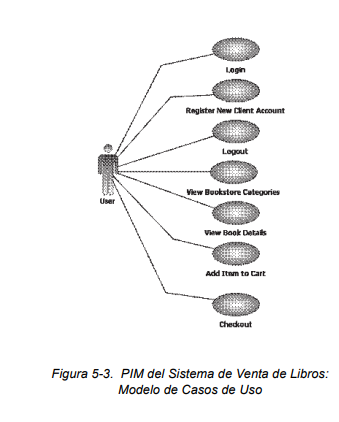
\includegraphics[scale=0.9]{./Imagenes/modelo22}
\caption{Ejemplo de figura 22}
\label{figura22}
\end{figure}


\subsection{5.3.2 Modelo estructural }

La figura 5-4 exhibe el diagrama de clases del sistema bookstore. Como puede verse en la figura, un bookstore tiene información acerca de sus clientes y de los libros que tiene en stock. Cada libro tiene una especificación de sus características y puede presentarse en dos versiones: digital o impreso. Los libros se organizan en categorías. Cada orden de compra está formada por varios ítems, donde se registra el ítem comprado, la cantidad y el precio pagado. Un usuario puede ir acumulando ítems en un carrito de compras y posteriormente efectivizar la compra de estos ítems. En la parte inferior de las figuras pueden verse definiciones escritas en OCL. Las primeras, por ejemplo, son las definiciones de dos operaciones en el contexto del carrito: getNumItems retorna la cantidad de elementos del carrito y getSubTotal retorna el total gastado.



\subsection{5.3.3 Modelos del comportamiento }

Para cada caso de uso se diseña un diagrama de secuencia mostrando la interacción de los elementos del sistema para llevar a cabo la funcionalidad pedida. Las figuras 5-5a-c muestran los diagramas que especifican el comportamiento del sistema bookstore para los casos de uso Login, Logout y View Book Details presentados anteriormente.

\begin{figure}[H]
\centering
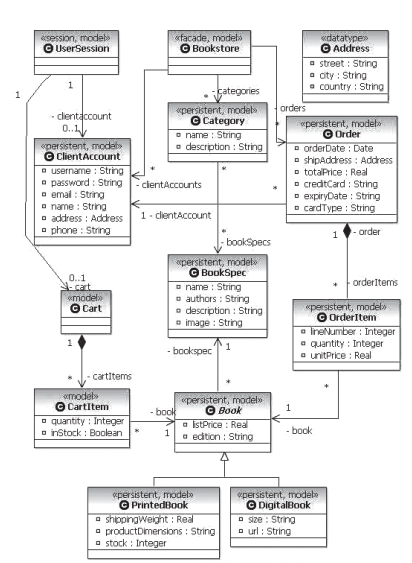
\includegraphics[scale=0.9]{./Imagenes/modelo23}
\caption{Ejemplo de figura 23}
\label{figura23}
\end{figure}
